\chapter{Conclusion and future work} \label{conclusionandfuturework}

\section{Conclusion}

Skylab is supposed to serve facilitators, advisers, mentors and students and potential students well by making experience in Orbital more pleasant. Through the whole process of Orbital program, Skylab has been playing a helpful role in registration, match making after registration, submissions of project log and README, peer evaluations for evaluated teams` submissions and feedback to peer evaluations. There is also quite some work done on admin portal for overseeing Skylab and reminding users and public views to display past projects and staff in Orbital program.

The development process of Skylab is certainly agile and iterative. Many features are developed as prototype first and after discussion adjustments are made to have a better user interaction experience. Besides, as Skylab is continuously being used, some requirements and suggestions are made by users as well. Many challenges to system design rise in the process of changing and refining. Various compromises have to be made to due to deadlines or other important issues. During implementation of Skylab, coping with changes and deadlines is the most important skill. Designing a system with enough features, with enough good features, with enough good features and extensibility to add more good features is huge challenge and Skylab is trying to be a system with many good features and open to extensions in the future.

\section{Achievements}

\subsection{Time and effort}

Skylab has been developed for over an year. Since March of 2015, various of issues and challenges have been conquered as achievements in the continuous implementation process. A recording of commit history of Skylab in GitHub is shown in Figure~\ref{fig:SkylabContribution}.

\begin{figure}[h]
  \centering
  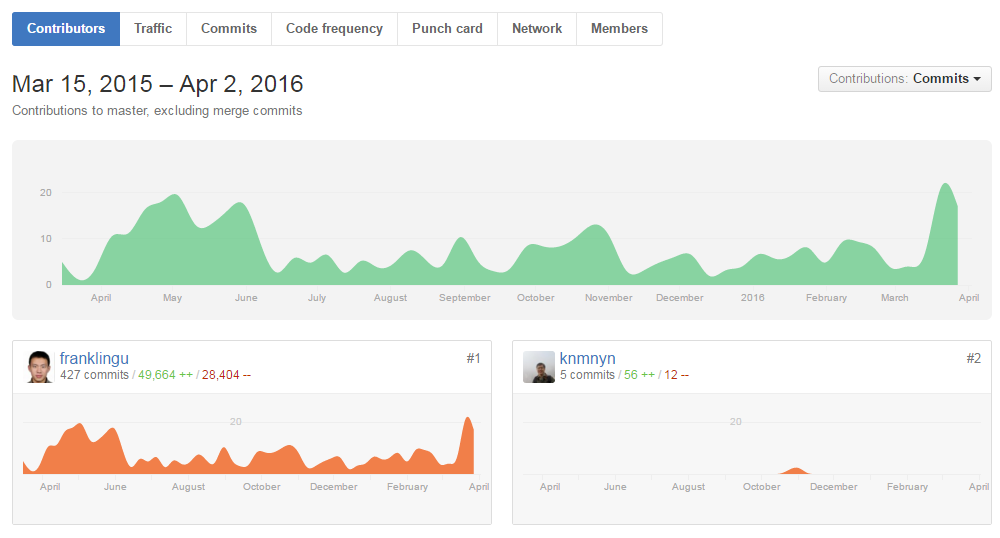
\includegraphics[width=\textwidth]{Images/Skylab_Contribution.png}
  \caption{Contribution history of Skylab}
  \label{fig:SkylabContribution}
\end{figure}

\subsection{Worked with Deadlines and Changes}

Just like any other software engineering projects, there are many deadlines during the process. And there will always be more requirements to complete, changes to expect along the way. Throughout the entire period of implementation of Skylab, working with deadlines and changes along the way is common and this brought many practical challenges to system design as well. A timeline diagram with all important milestones is as Figure~\ref{fig:SkylabTimeline}.

\begin{figure}[h]
  \centering
  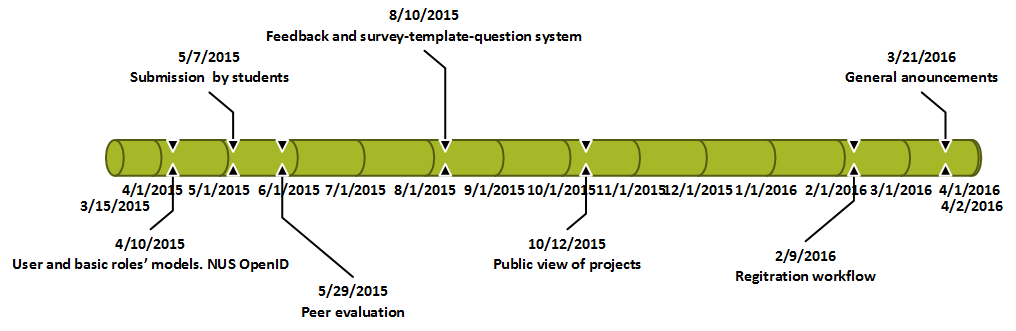
\includegraphics[width=\textwidth]{Images/Skylab_Timeline.png}
  \caption{Timeline of Skylab}
  \label{fig:SkylabTimeline}
\end{figure}

\subsection{Live Server Setup and Maintenance}

Skylab is first hosted on an Amazon EC2 instance and later migrated to NUS SoC virtual machine. About 400 users are using Skylab to carry out different activities based on their roles. Also at times some maintenance work may be needed on production server to release new versions of Skylab.

\subsection{Development Process}

GitHub workflow has been well adopted in the development of Skylab and it is agile and iterative. Also with continuous integration tool like Travis, code quality and test coverage monitoring tool like CodeClimate, security analysis tool like Hikiri, the whole process is more smooth and different issues could be watched on the go.

\subsection{Major Use Cases}

Skylab is designed to serve all kinds of people involved in Orbital and it has been working great to support Orbital program. From registration phase of Orbital program to last feedback in Orbital, Skylab is playing a major role in helping admins, advisers, mentors, tutors and students.

\begin{itemize}
  \item Registration: students who are interested in Orbital can sign up via Skylab. They can do this as a team of two or as individuals first. For those individuals, a match making algorithm will be run to find potential teammates based on recorded interested topics of each student.
  \item Evaluation: students and advisers will go through evaluation process in Orbital which includes submissions, peer evaluations and feedback.
  \item Administration: admins can overview things in Skylab.
  \item Mailing: various emails as reminders can be sent through Skylab.
  \item Public facing of profiles: staff of Orbital, past projects of Orbital can be displayed in Skylab easily.
\end{itemize}

\section{Future work}

A proposed set of major features to be completed in the future for Skylab:

\begin{itemize}
  \item Questions/template system(involving migration of current data): currently \textit{Feedback} and \textit{Peer Evaluation} is utilizing the \textit{SurveyTemplate} and \textit{Question} system but \textit{Submission} are still not. With migration to \textit{Questions} system we can further improve the system by adding more extensibility.
  \item Logging of user activities: by logging down activities carried out by different users, users can more easily figure out what has happened and get a better sense of the context of Skylab.
  \item Unit testing need to cover more classes and acceptance testing needs cover more use cases in Skylab by different users.
\end{itemize}

